\newpage
\chapter{Diagramas}
\label{chap:diagrams}
La herramienta no hace un uso intensivo de la orientación a objetos, en lo referente a herencia, composición, clases abstractas y similares. No obstante sí que existe una jerarquía de objetos de almacenamiento y representación de los hechos lógicos representados a la salida de los diferentes módulos. Con respecto al diagrama de secuencia, su ausencia es justificable ya que no ilustra nada ni sirve a ningún propósito real. El diagrama de arquitectura aclara mucho mejor el funcionamiento y el flujo de datos entre los módulos del sistema que cualquier diagrama de secuencia, ya que los diferentes módulos se invocan secuencialmente y la salida de cada uno se recibe en el pipeline y se pasa al siguiente módulo hasta terminar.

\begin{figure}[th]
	\centering
	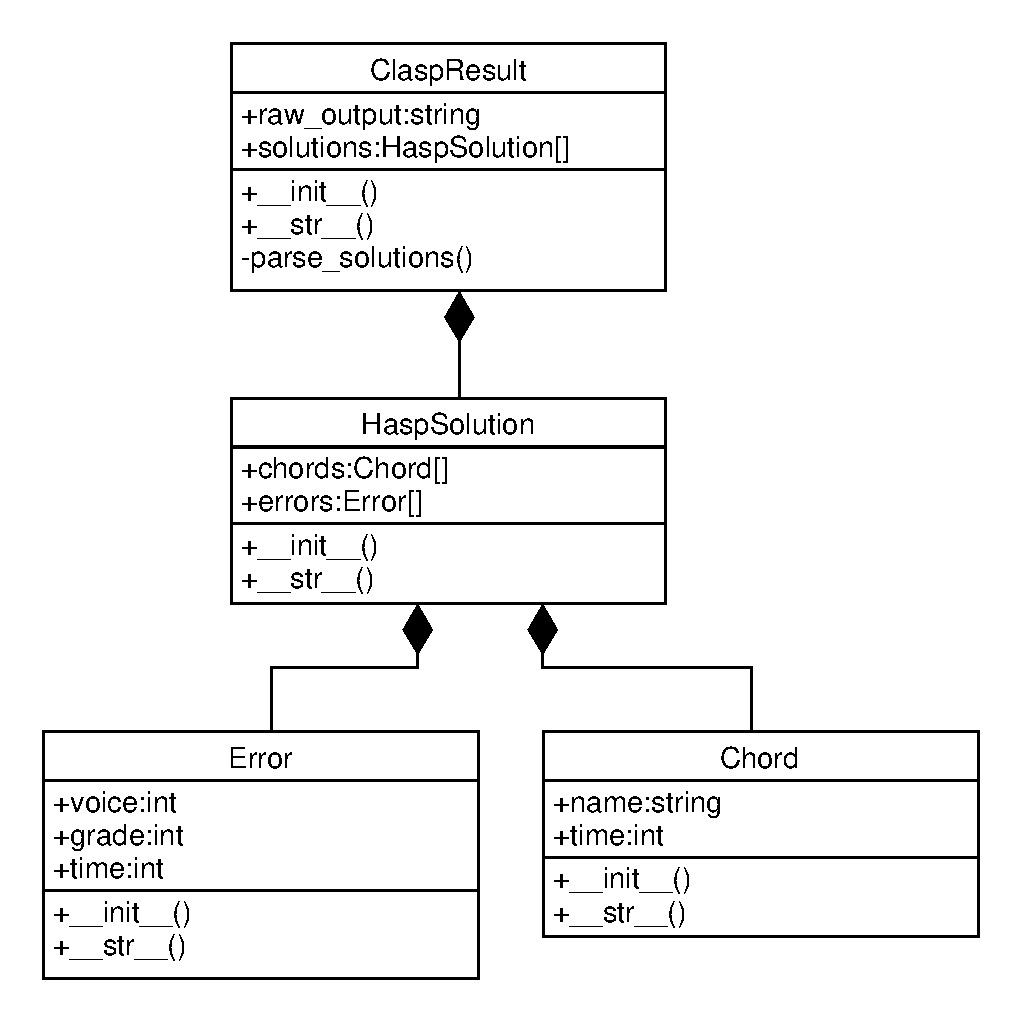
\includegraphics[width=0.8\linewidth]{imagenes/third_iter.pdf}
	\caption{Diagrama de clases de almacenamiento de la Iteración 3}
	\label{fig:class_diagram_third}
\end{figure}
\newpage
\begin{figure}[th]
	\centering
	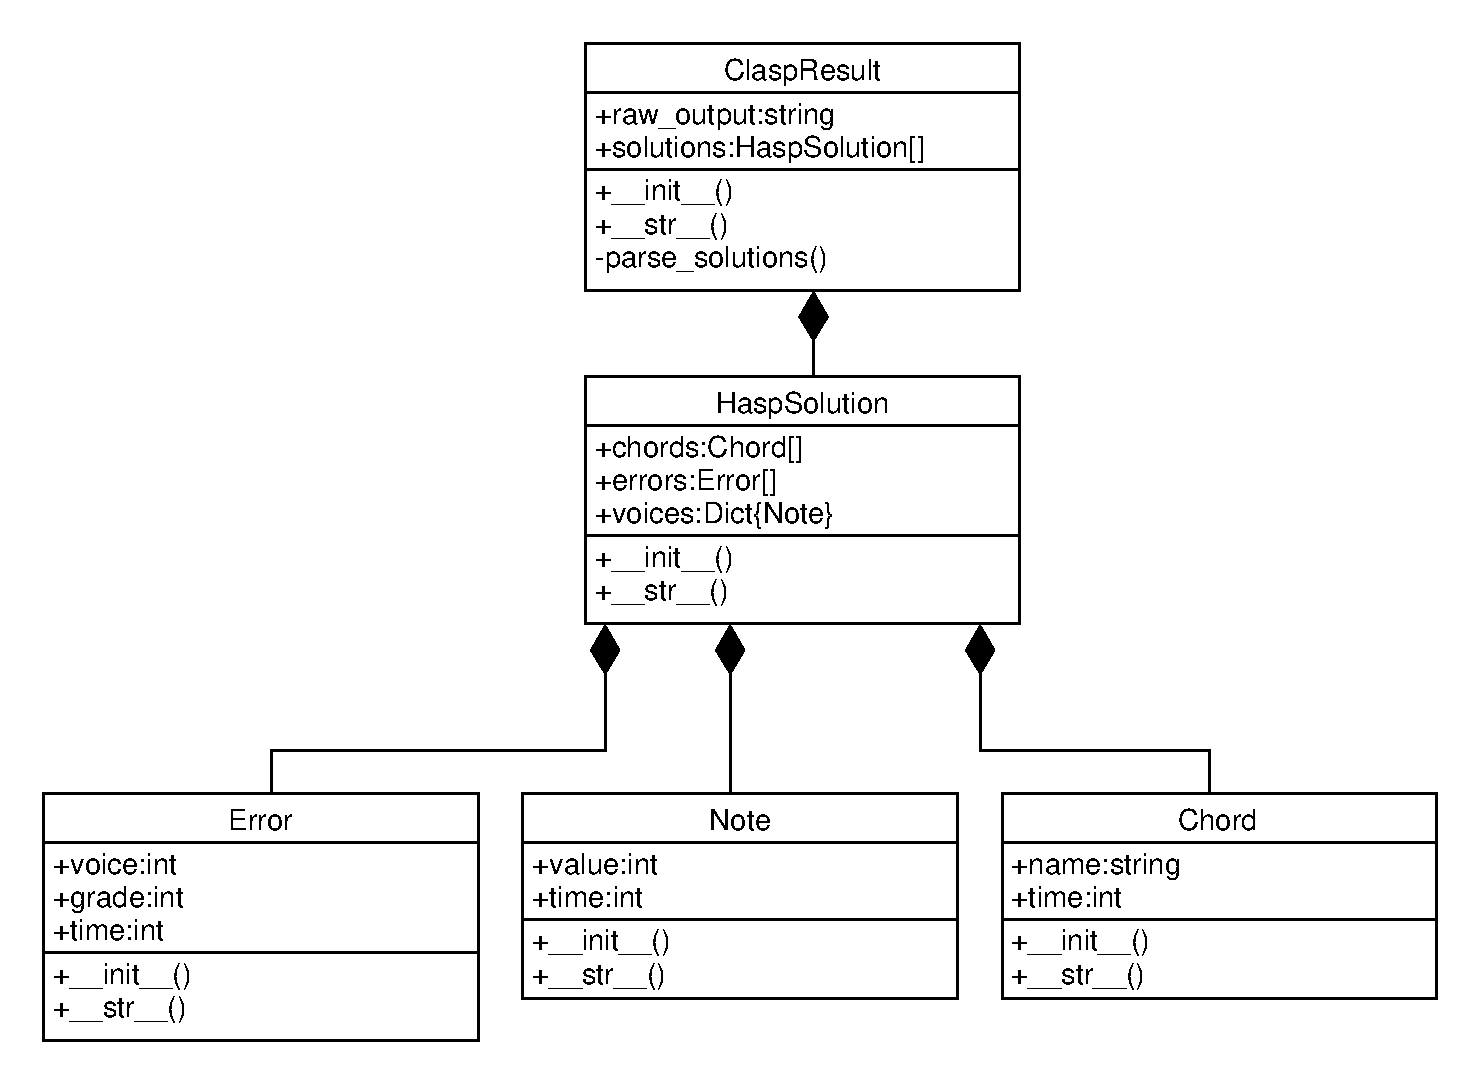
\includegraphics[width=0.8\linewidth]{imagenes/fourth_iter.pdf}
	\caption{Diagrama de clases de almacenamiento de la Iteración 4}
	\label{fig:class_diagram_fourth}
\end{figure}
\begin{figure}[th]
	\centering
	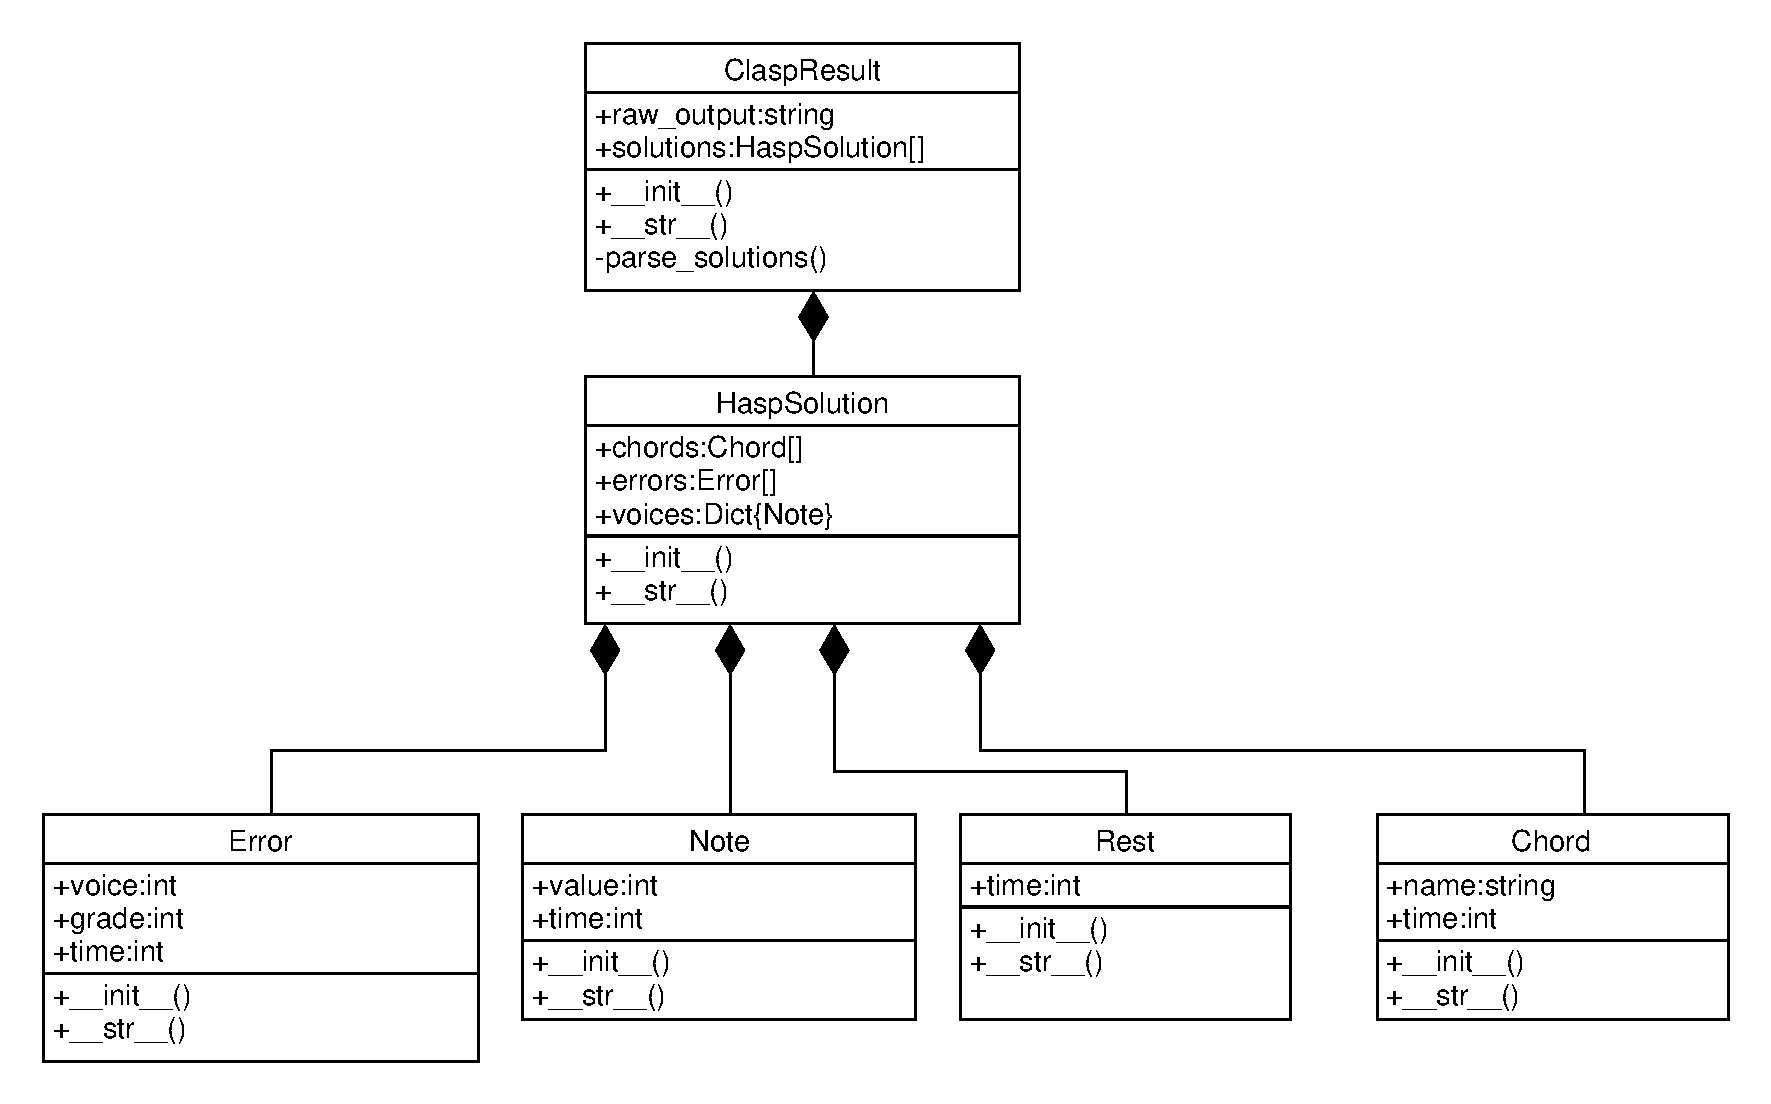
\includegraphics[width=0.8\linewidth]{imagenes/fifth_iter.pdf}
	\caption{Diagrama de clases de almacenamiento de la Iteración 5}
	\label{fig:class_diagram_fifth}
\end{figure}
\begin{figure}[th]
	\centering
	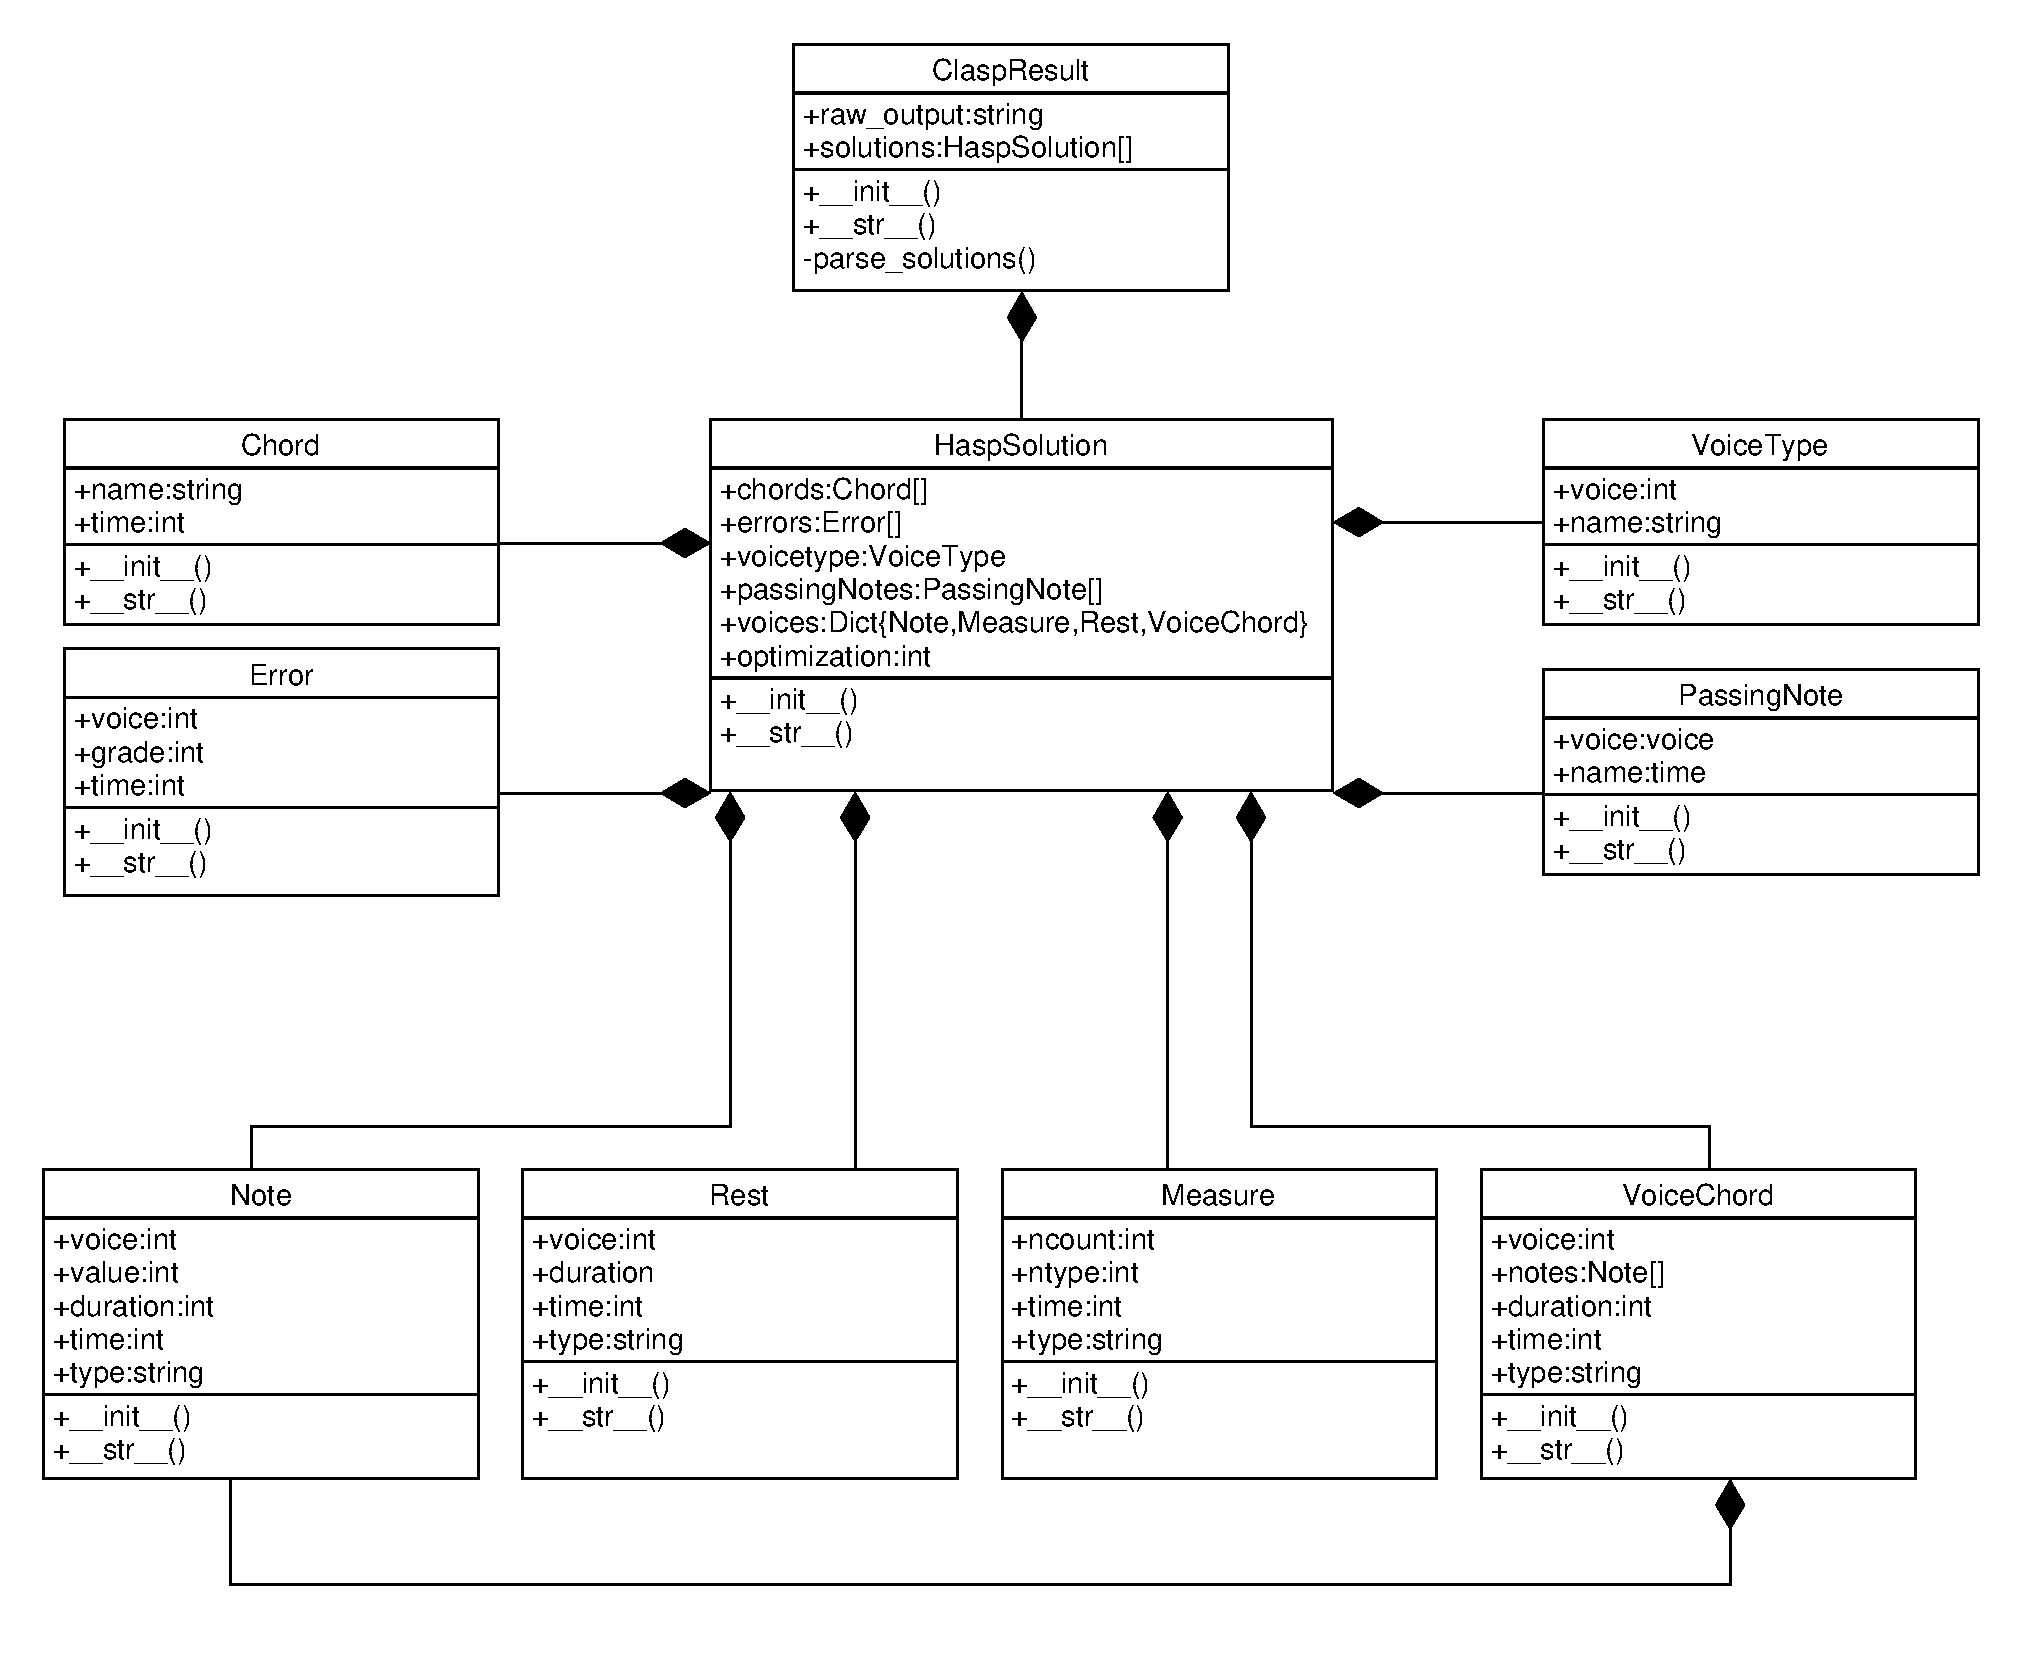
\includegraphics[width=0.8\linewidth]{imagenes/sixth_seventh_eighth_iters.pdf}
	\caption{Diagrama de clases de almacenamiento de las Iteraciones 6, 7 y 8}
	\label{fig:class_diagram_sixth_seventh_eighth}
\end{figure}
\begin{figure}[th]
	\centering
	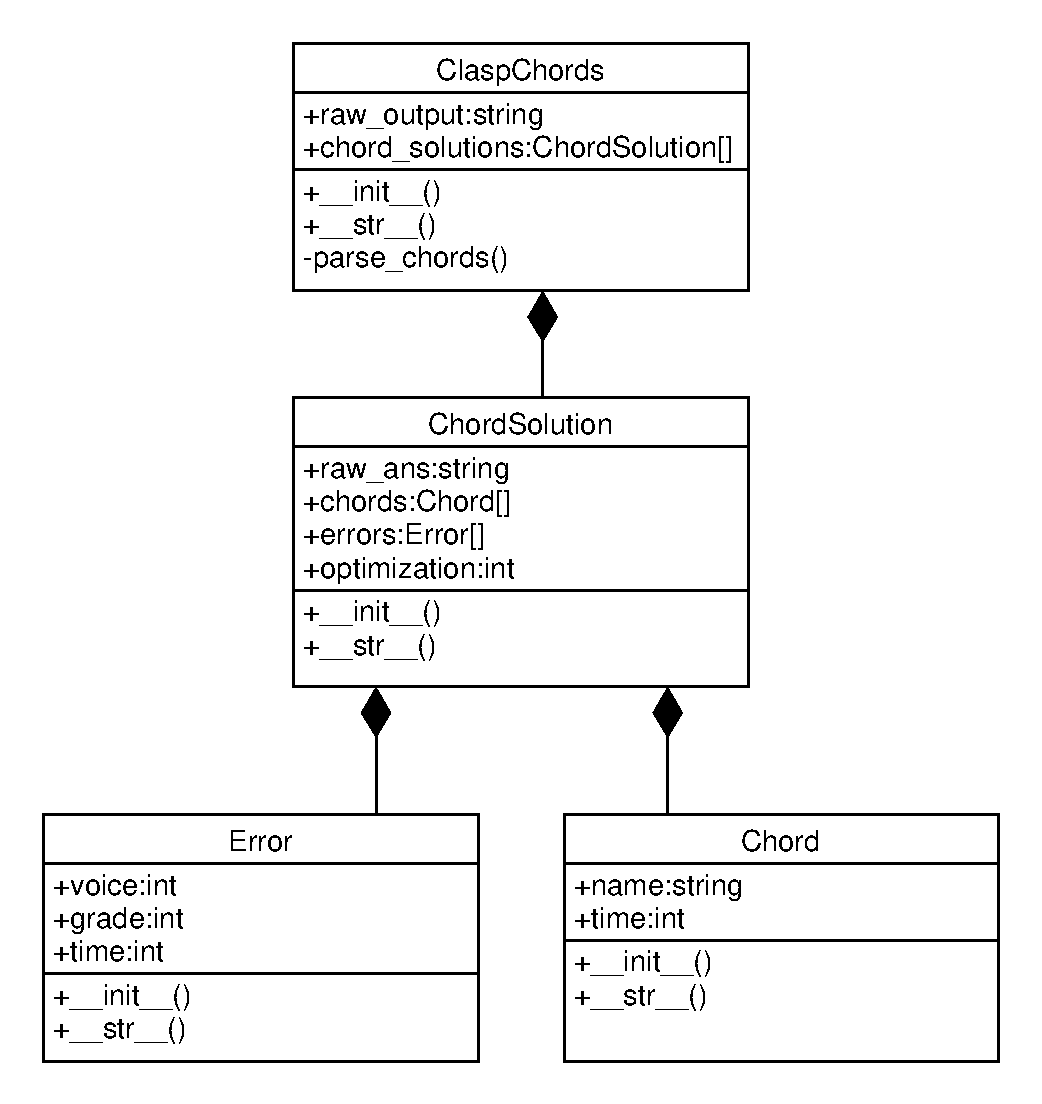
\includegraphics[width=0.8\linewidth]{imagenes/chord_diagram.pdf}
	\caption{Diagrama de clases de almacenamiento del módulo de armonización de la iteración 8}
	\label{fig:class_diagram_chords}
\end{figure}

\chapter{Análisis de MusicXML}
\label{chap:musicxml_analysis}
Se detalla una relación de los elementos MusicXML identificados por el procesador y se especifica la finalidad de los mismos. Se indica también, el tipo de cada elemento procesado (Etiqueta, Etiqueta Autocerrada o Atributo) y, con fines organizativos, la etiqueta con la que están relacionados de forma directa.

 \begin{center}
 	\newcommand*{\TitleParbox}[1]{\parbox[c]{1.75cm}{\raggedright #1}}%
 	\begin{longtable}{ | l | c | c | p{6.5cm} | }
 		\hline
 		Nombre & Pertenece a & Tipo & Uso \\ \hline \hline
 		note & measure & Etiqueta & Delimita el bloque correspondiente a una nota o silencio \\ \hline
 		step & note & Etiqueta &  Especifica el nombre de la nota en notación internacional \\ \hline
 		octave & note & Etiqueta &  Indica el número de la octava de la nota \\ \hline
 		rest & note & Autocerrada & Indica si la figura es un silencio, en caso de aparecer, step y octave no se especifican \\ \hline
 		chord & note & Autocerrada & Indica si la nota forma parte de un acorde \\ \hline
 		type & note & Etiqueta & Especifica el tipo de figura mediante un string (whole, half, quarter...) \\ \hline
 		staff & note & Etiqueta & Identifica el número de pentagrama al que pertenece la nota, usado en instrumentos con múltiples pentagramas como el piano \\ \hline
 		grace & note & Autocerrada & Indica si la nota es una apoyatura \\ \hline
 		alter & note & Etiqueta & Especifica el valor de alteración usando números positivos para sostenidos y negativos para bemoles \\ \hline
 		duration & note & Etiqueta & Indica la duración de la figura \\ \hline
 		dot & note & Autocerrada & Indica si la nota está acompañada de un puntillo \\ \hline
 		part & score-partwise & Etiqueta & Delimita los bloques de cada voz o parte de la partitura \\ \hline
 		score-part & part-list & Etiqueta & Delimita los bloques de meta-información de cada una de las partes \\ \hline
 		instrument & score-part & Etiqueta & Especifica el nombre del instrumento la parte correspondiente \\ \hline
 		print-object & note & Atributo & Indica si la nota es visible o no \\ \hline
 		credit-words & credit & Etiqueta & Almacena metadatos sobre autor o título de la partitura \\ \hline
 		time & attributes & Etiqueta & Delimita bloques sobre la información de compases \\ \hline
 		beats & time & Etiqueta & Indica la cantidad de figuras del compás (numerador) \\ \hline
 		beat-type & time & Etiqueta & Indica la figura base del compás (denominador) \\ \hline
 		harmony & measure & Etiqueta & Delimita un bloque que especifica la notación de armonía del compás \\ \hline
 		root-step & harmony & Etiqueta & Indica la nota raíz del acorde que se anota sobre el compás \\ \hline
 		kind & harmony & Etiqueta & Indica el tipo de acorde anotado sobre el compás (mayor, menor, dominante séptima...) \\ \hline
 		fifths & key & Etiqueta & Indica la cantidad de sostenidos o bemoles presentes en la armadura de la partitura. Usa números positivos para los sostenidos y negativos para los bemoles \\ \hline
 		mode & key & Etiqueta & Indica el modo (mayor o menor) de la tonalidad especificada por la armadura de la partitura \\ \hline
 	\end{longtable}
 \end{center} 
 
 \chapter{Partituras}
 \label{chap:scores}
 Además de las utilizadas en la evaluación del sistema, se utilizaron algunas otras partituras durante el desarrollo del proyecto, algunas descartadas por incompatibilidad y otras por no servir de ejemplo para la evaluación.
 
 \begin{figure}
 	\centering
 	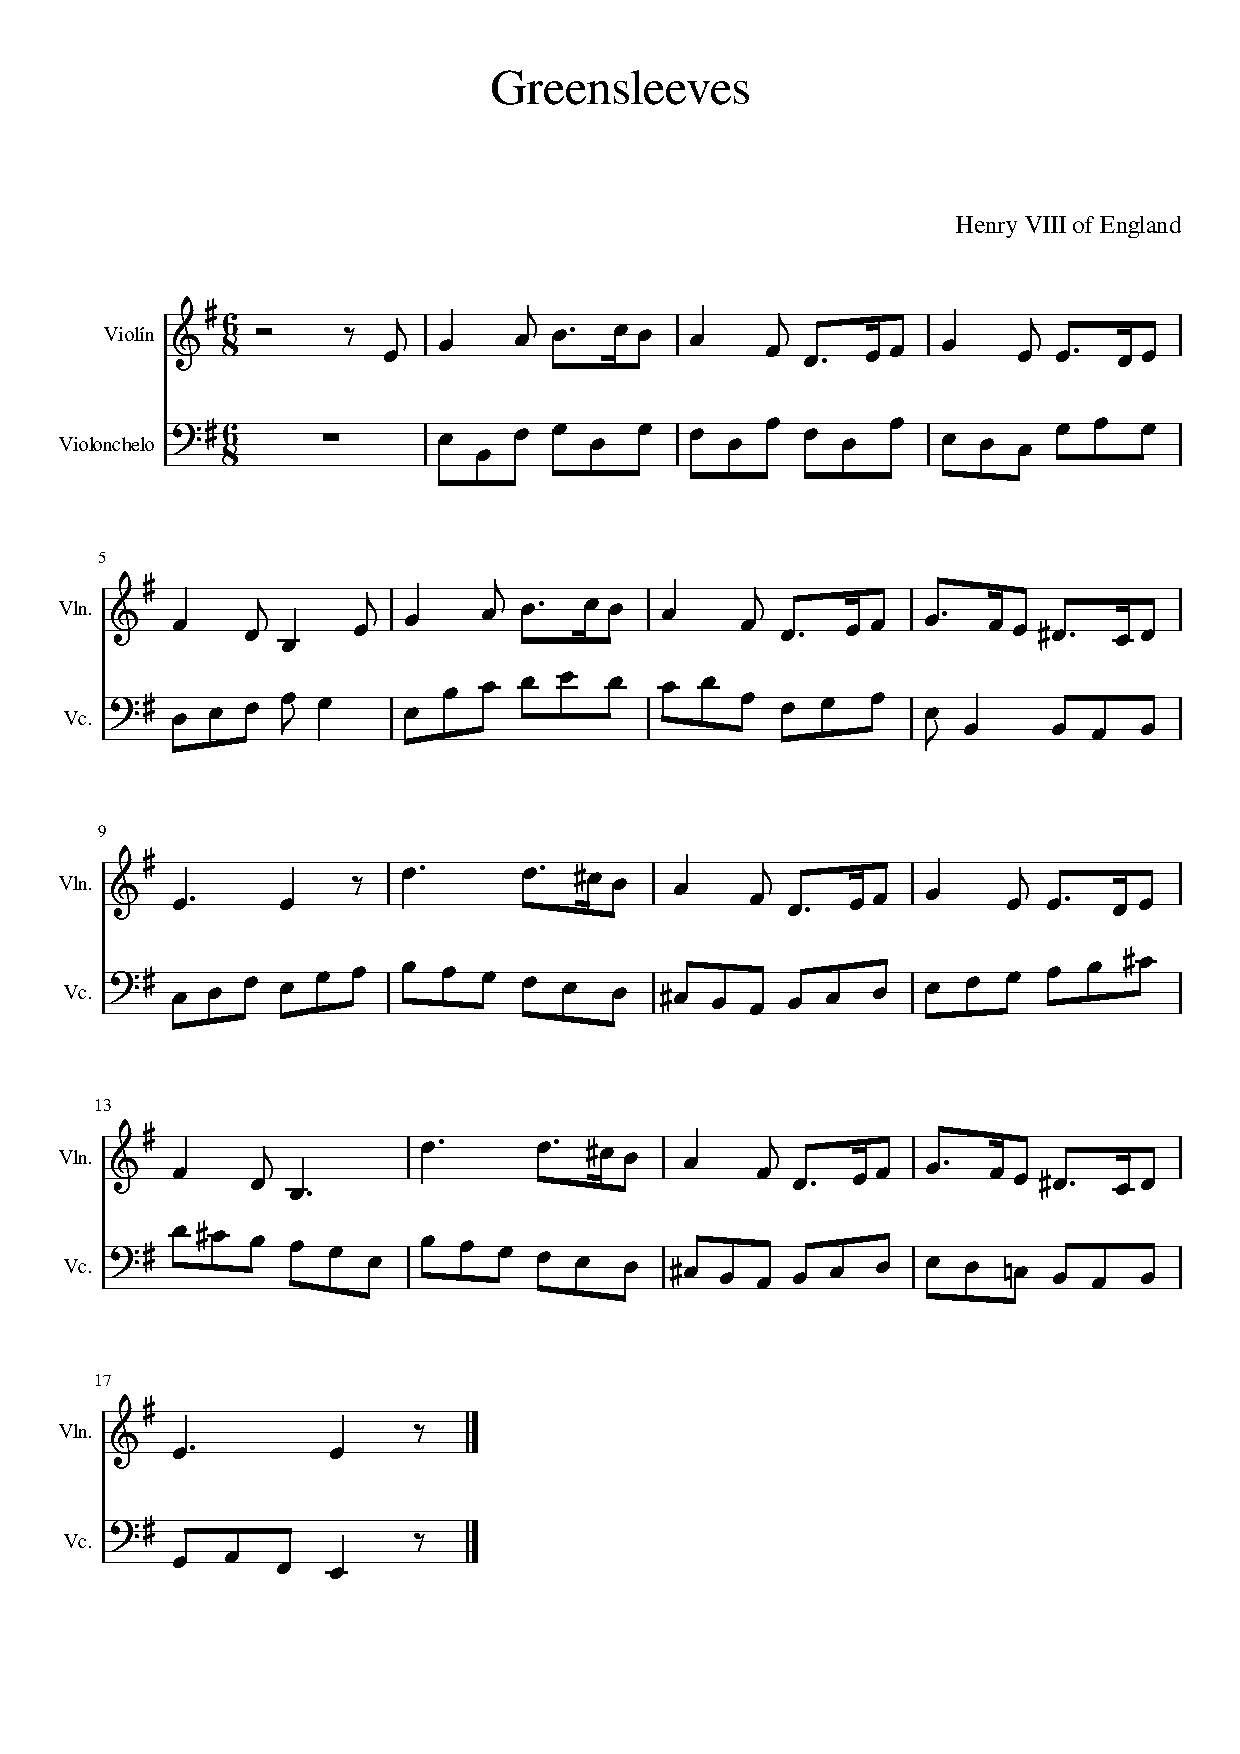
\includegraphics[width=0.8\linewidth]{imagenes/scores/Greensleeves.pdf}
 	\caption{Partitura de Greensleeves, por Enrique VIII}
 	\label{fig:greensleeves_score}
 \end{figure}
 
  \begin{figure}
  	\centering
  	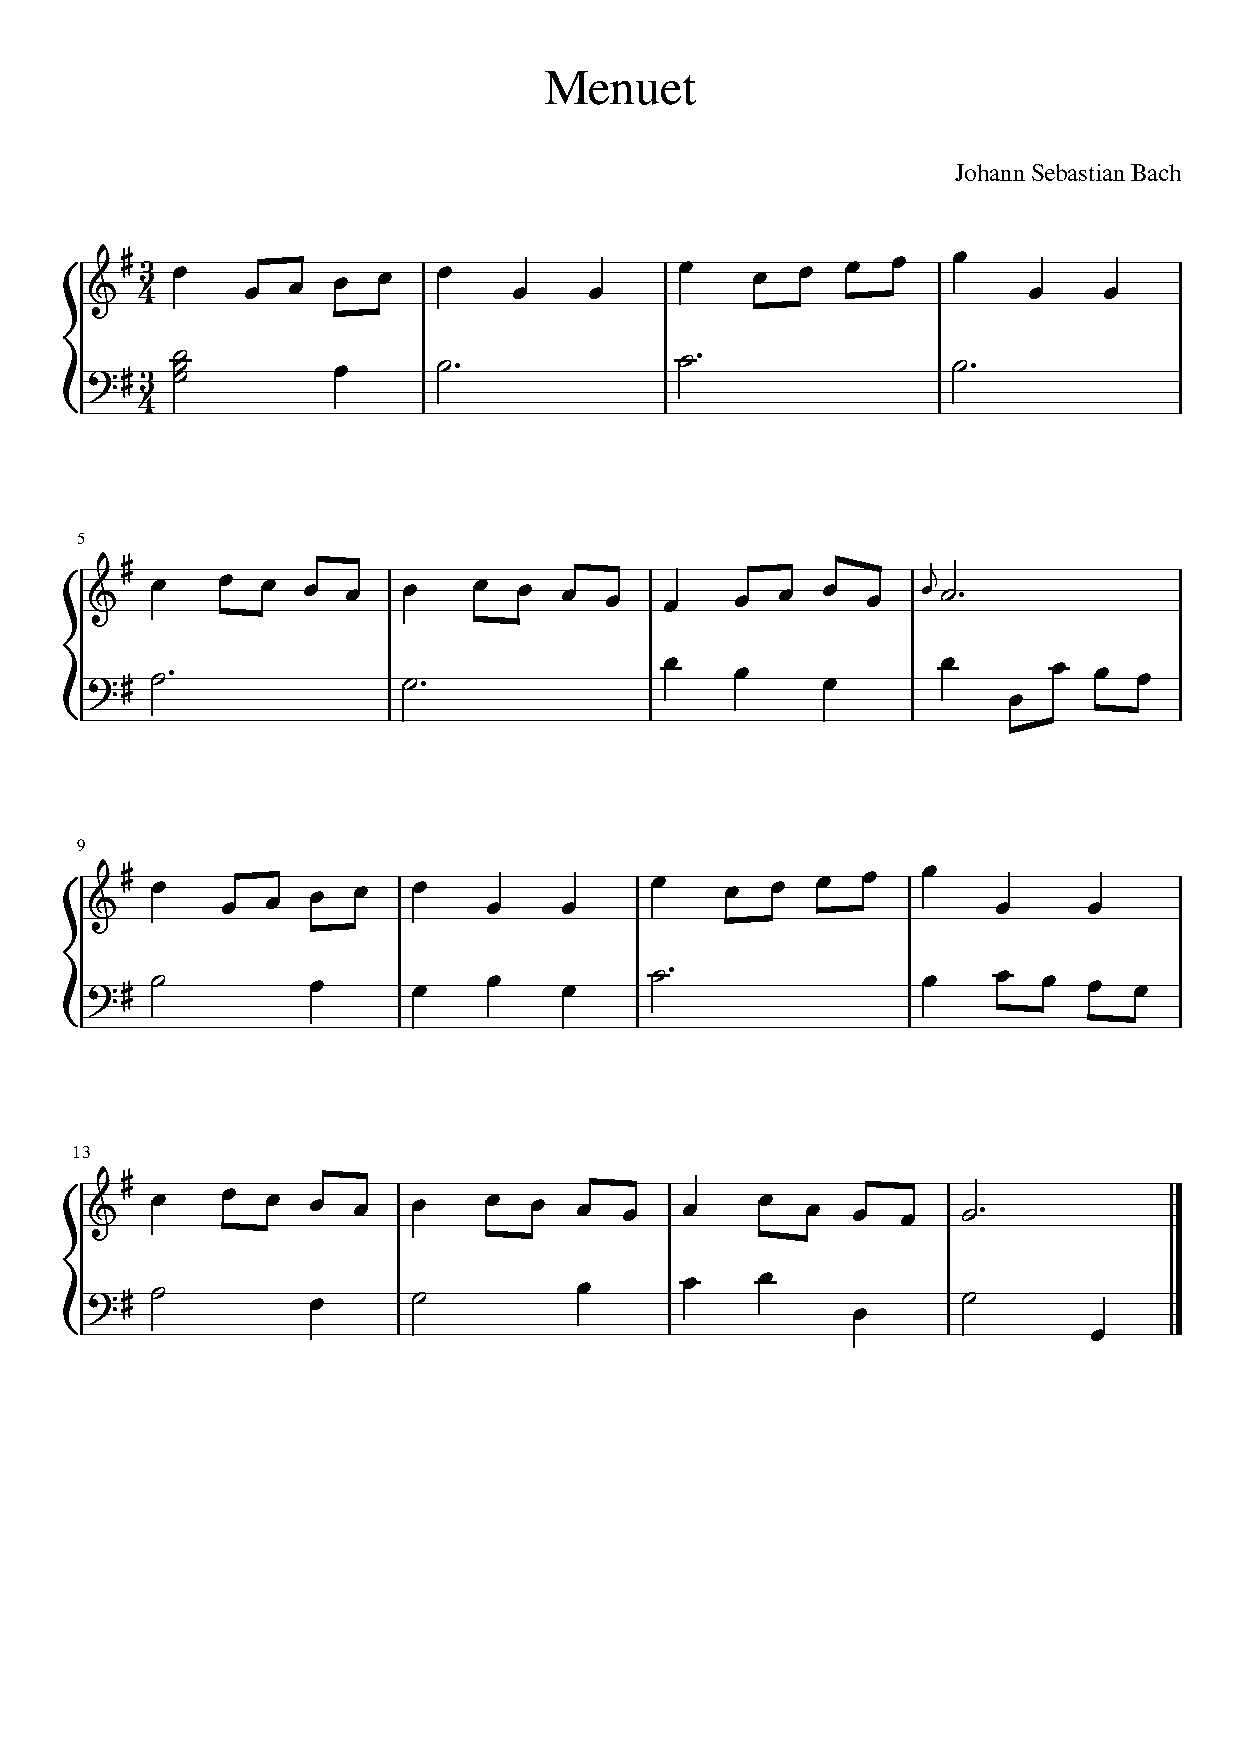
\includegraphics[width=0.8\linewidth]{imagenes/scores/menuet_bach.pdf}
  	\caption{Partitura de Menuet, por Johann S. Bach}
  	\label{fig:menuet_score}
  \end{figure}
  
    \begin{figure}
    	\centering
    	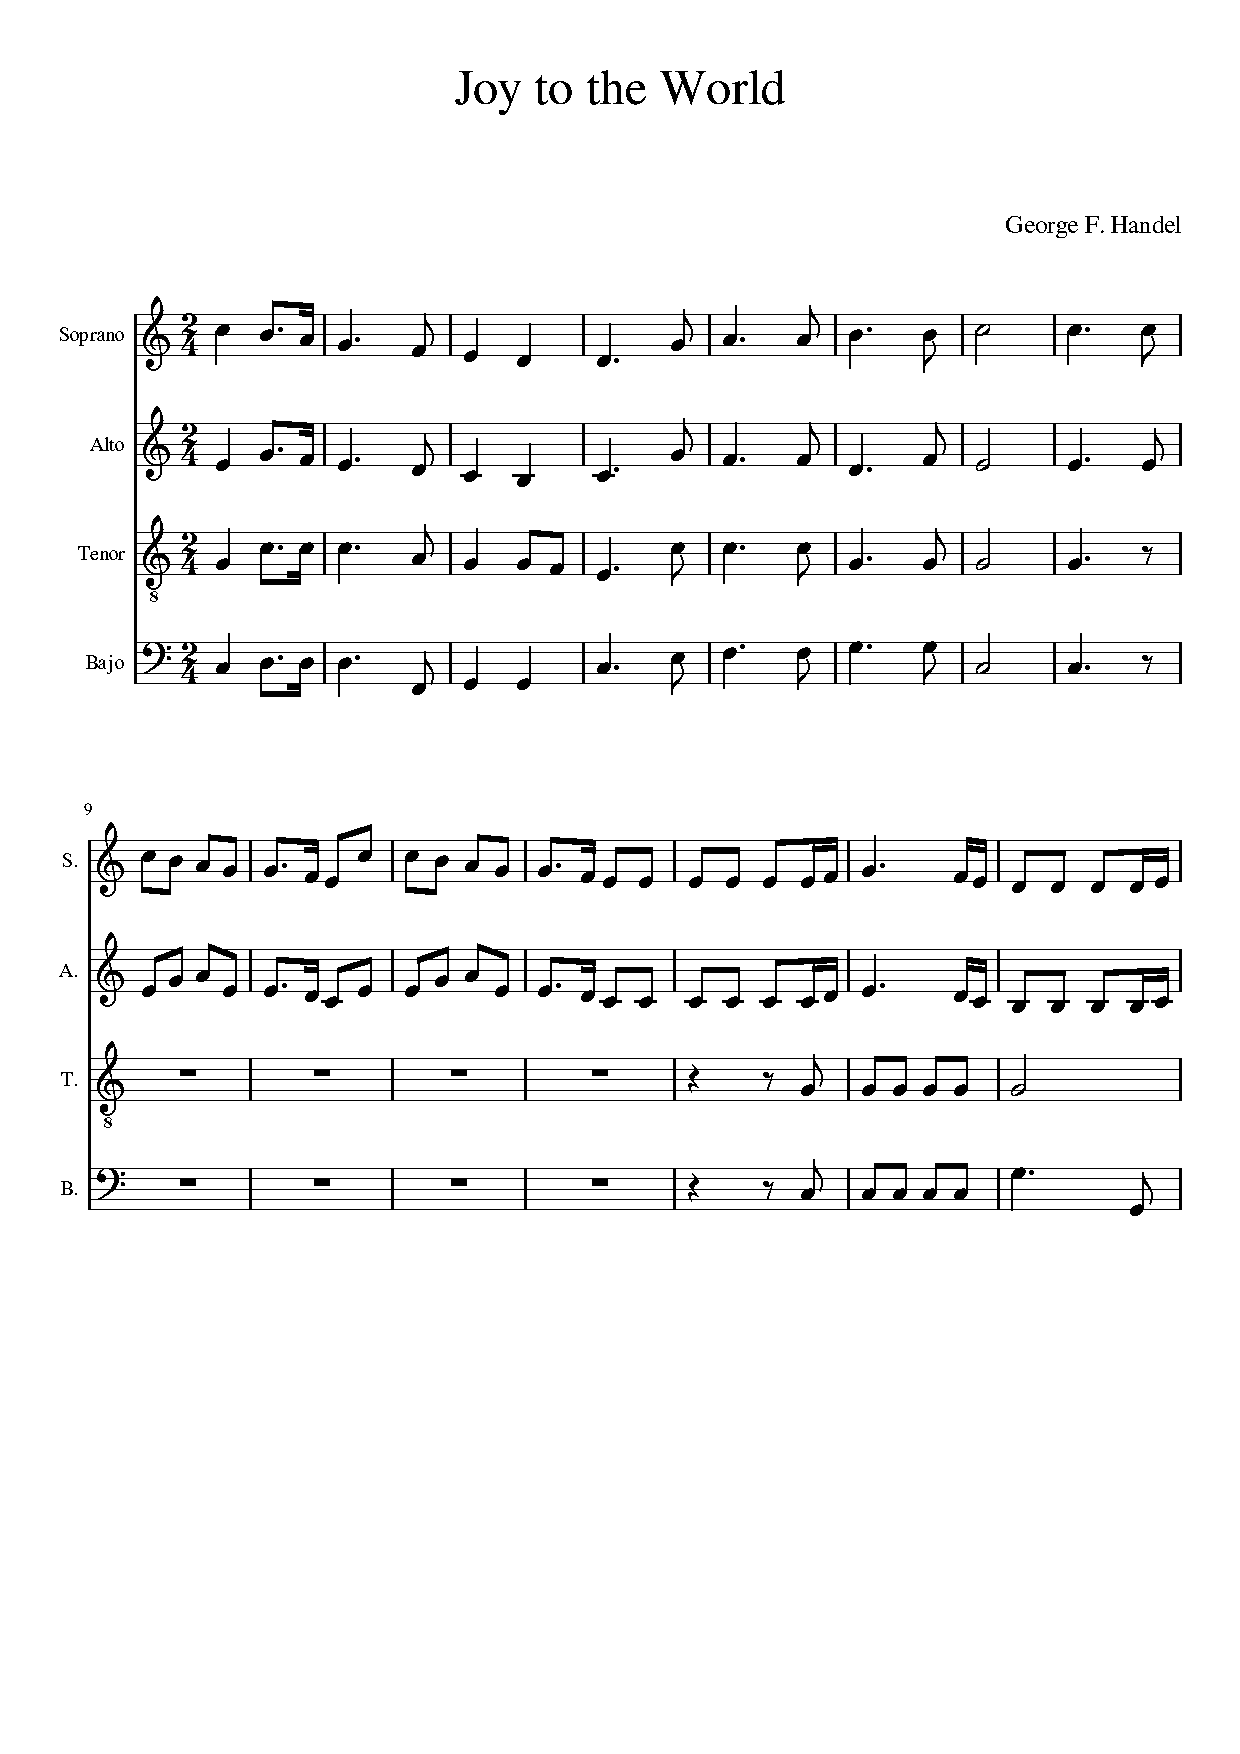
\includegraphics[width=0.8\linewidth]{imagenes/scores/Joy_to_the_World.pdf}
    	\caption{Partitura de Joy to the World, por George F. Handel}
    	\label{fig:joy_score}
    \end{figure}
 
     \begin{figure}
     	\centering
     	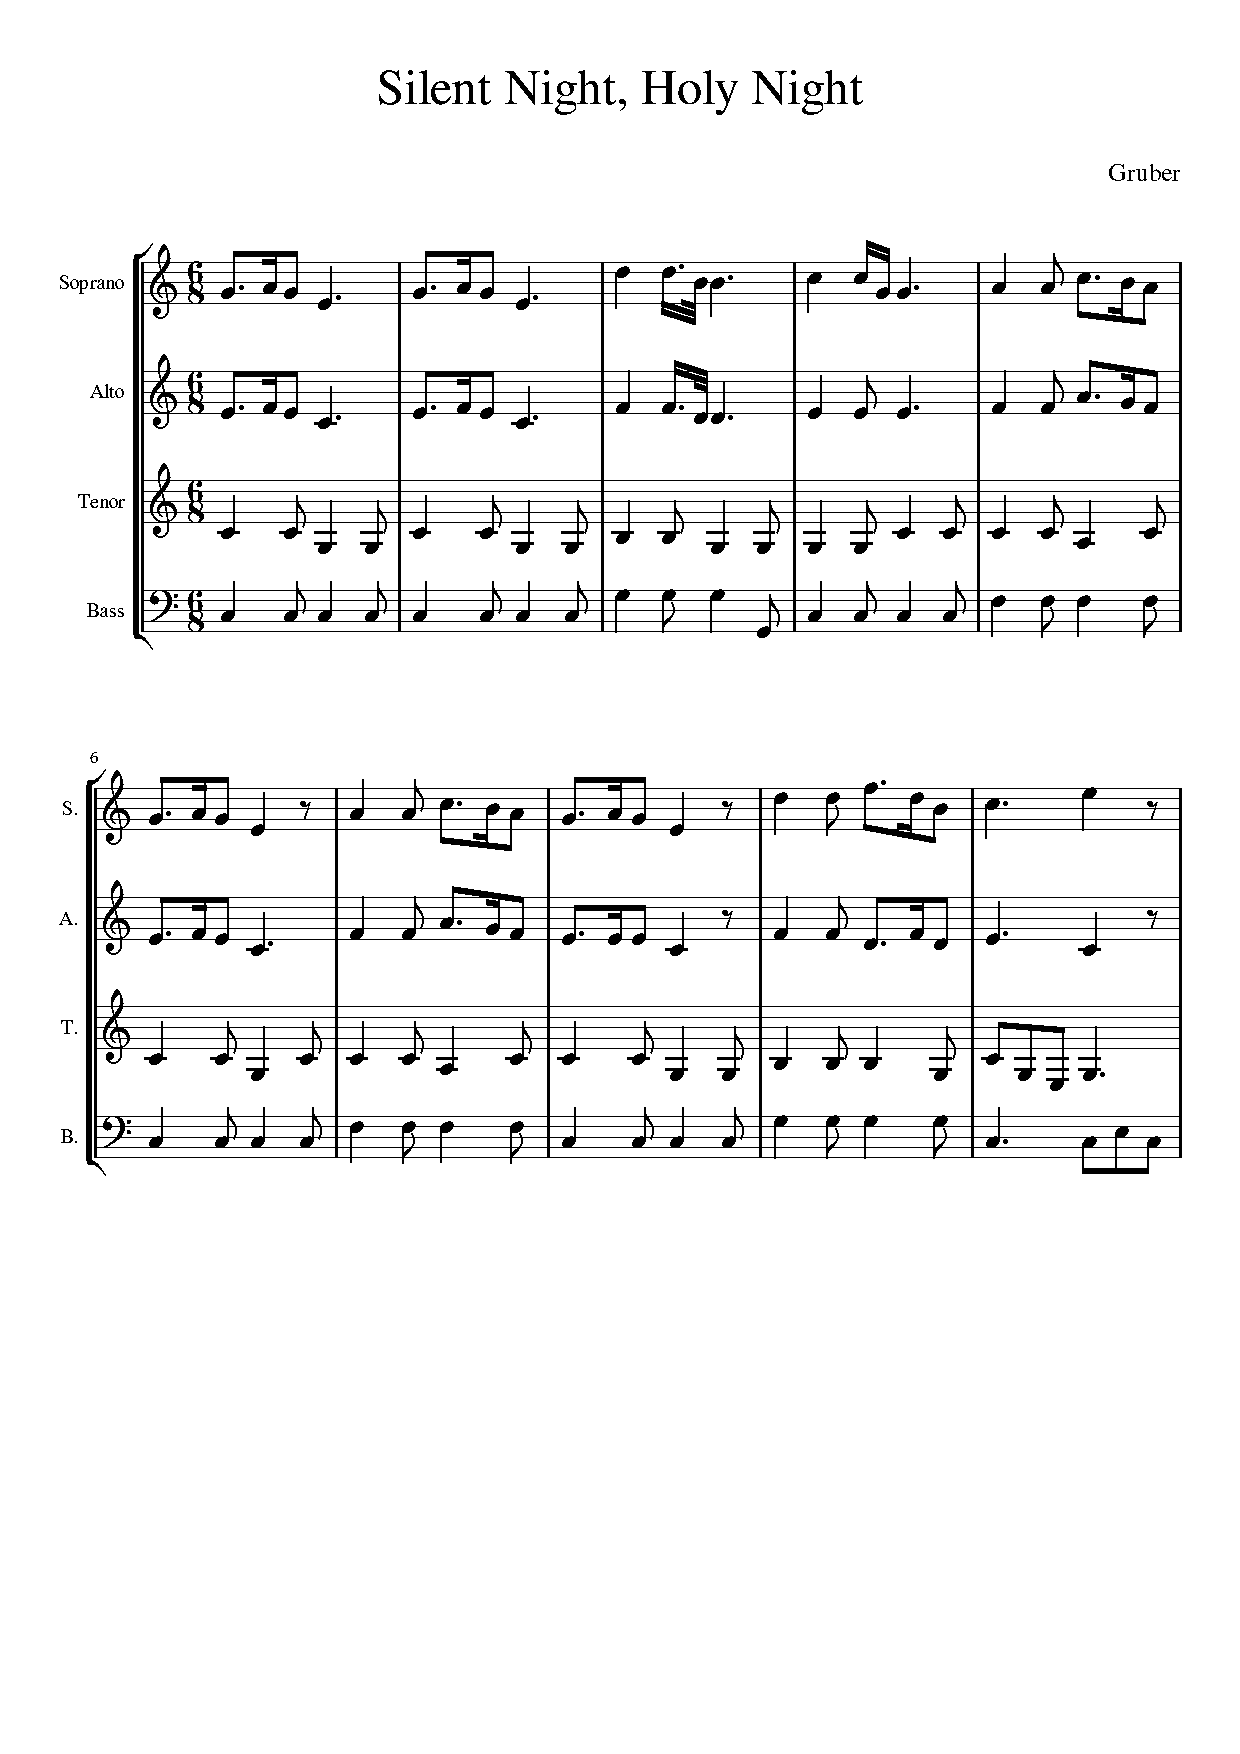
\includegraphics[width=0.8\linewidth]{imagenes/scores/silent_night.pdf}
     	\caption{Partitura de Silent Night (Noche de Paz), por Franz X. Gruber}
     	\label{fig:silent_score}
     \end{figure}
     
          \begin{figure}
          	\centering
          	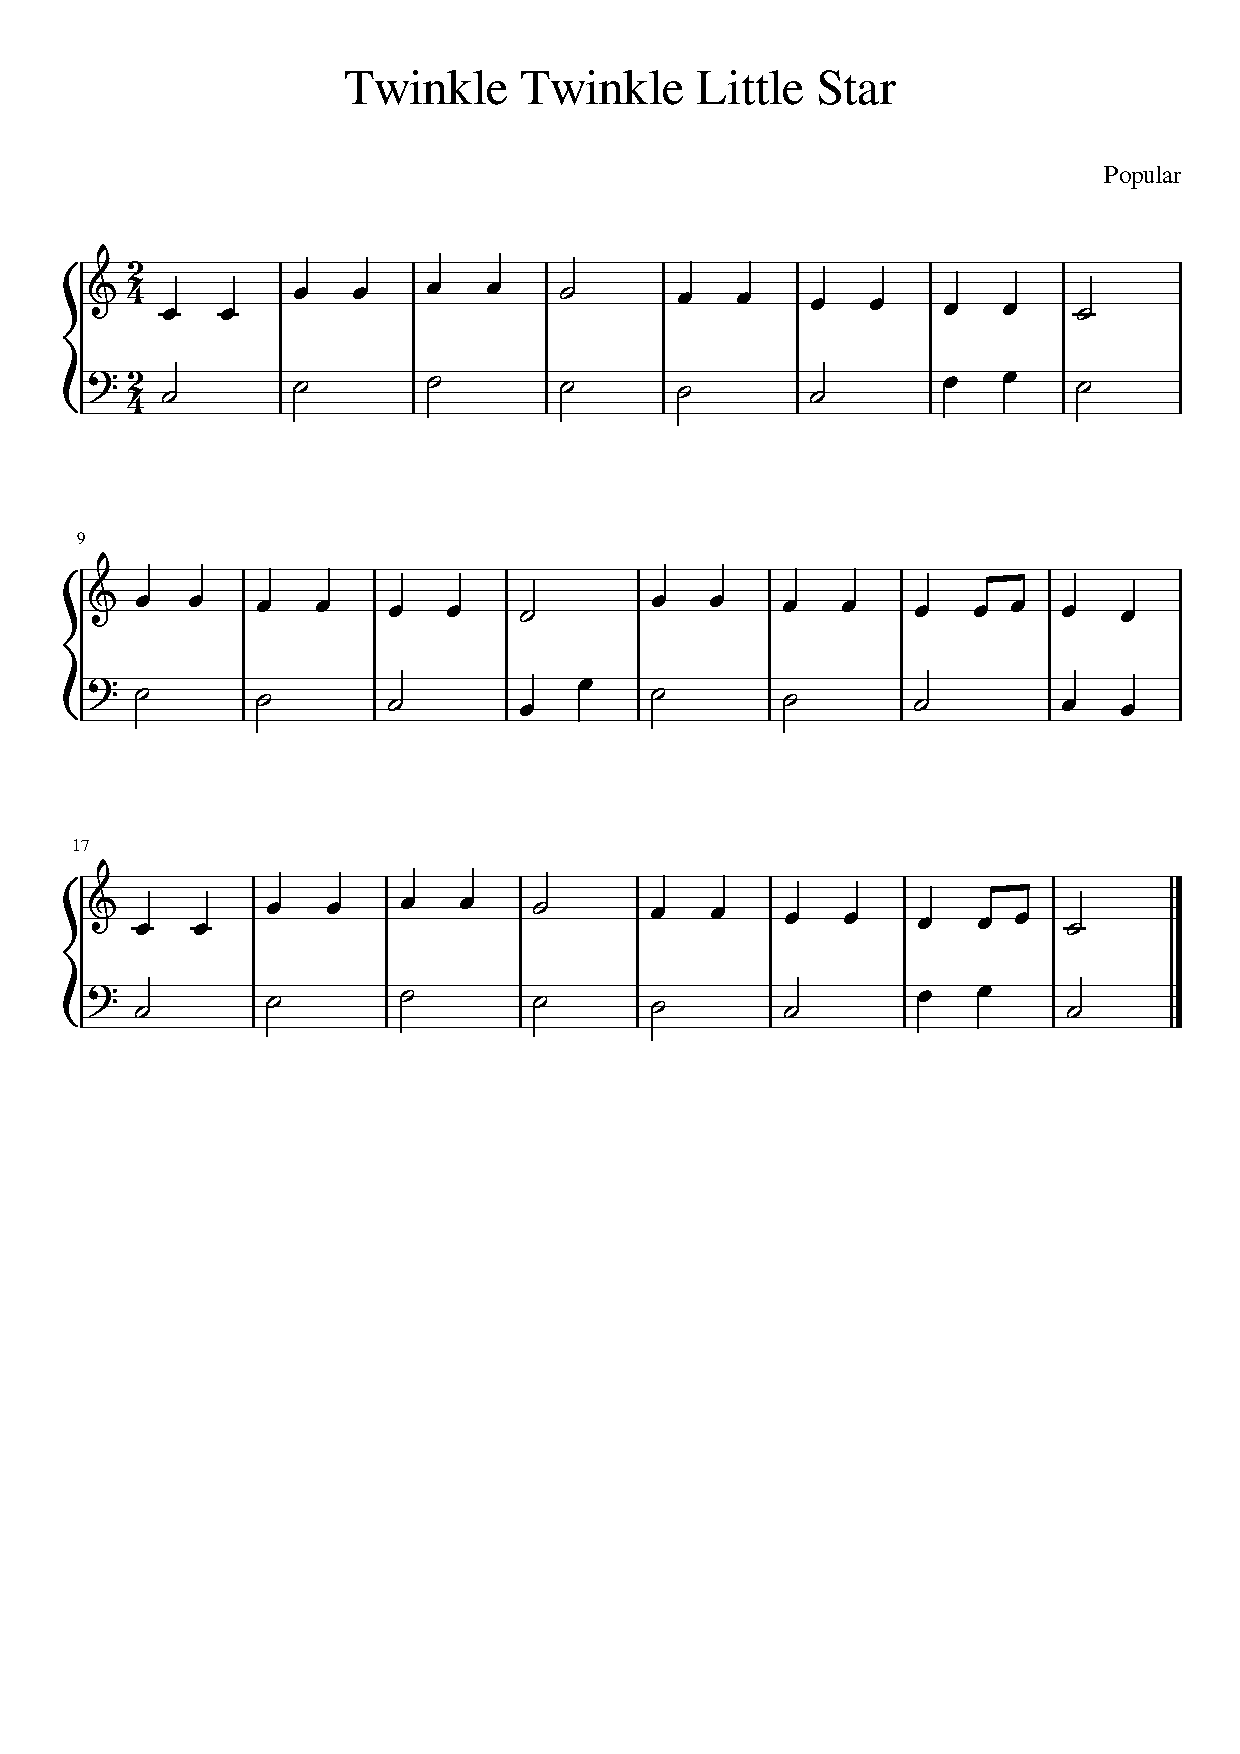
\includegraphics[width=0.8\linewidth]{imagenes/scores/Twinkle_Twinkle_Little_Star.pdf}
          	\caption{Partitura de la pieza popular infantil Twinkle Twinkle Little Star (Brilla Brilla Estrellita)}
          \end{figure}
     
     \begin{figure}
     	\centering
     	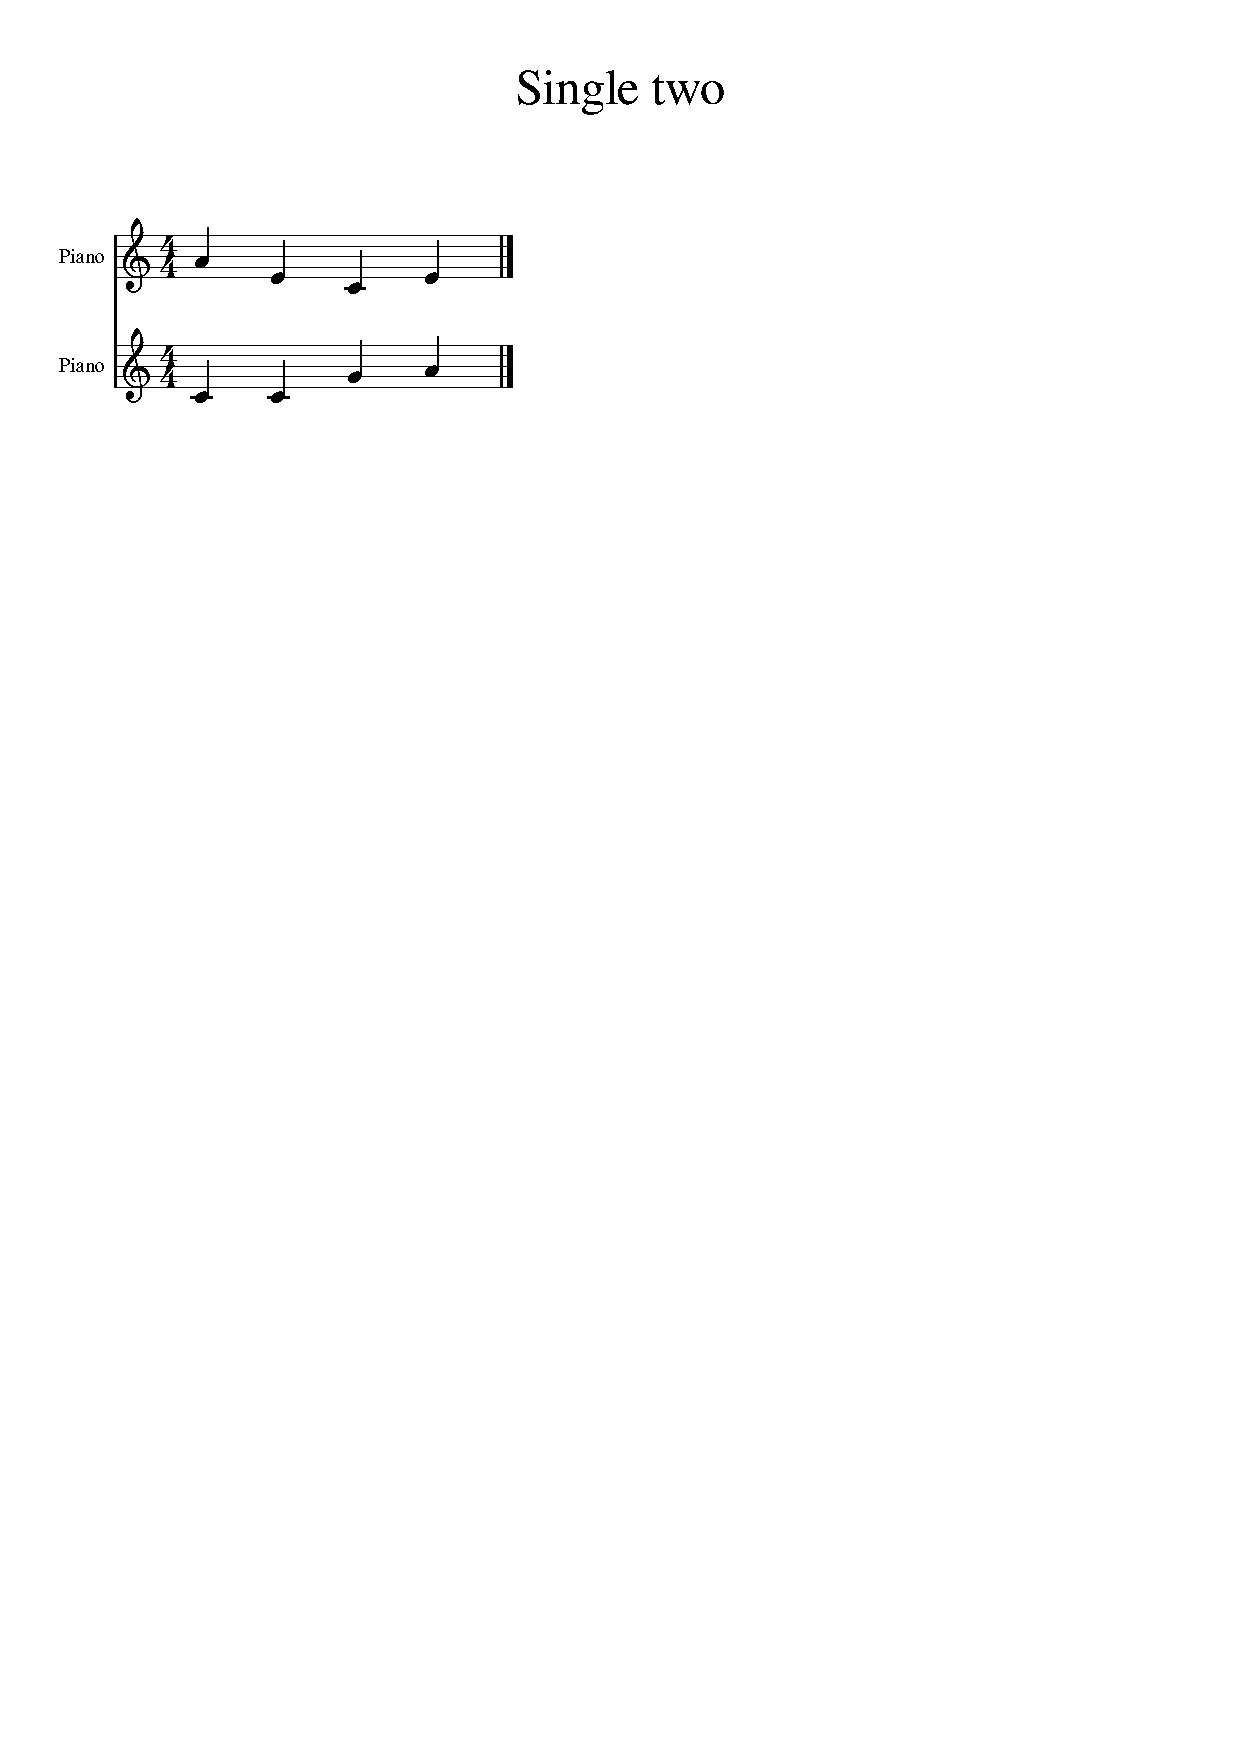
\includegraphics[width=0.8\linewidth]{imagenes/scores/simple_chords.pdf}
     	\caption{Partitura de ejemplo con una serie de acordes sencillos}
     	\label{fig:simplechords_score}
     \end{figure}

 \begin{figure}
 	\centering
 	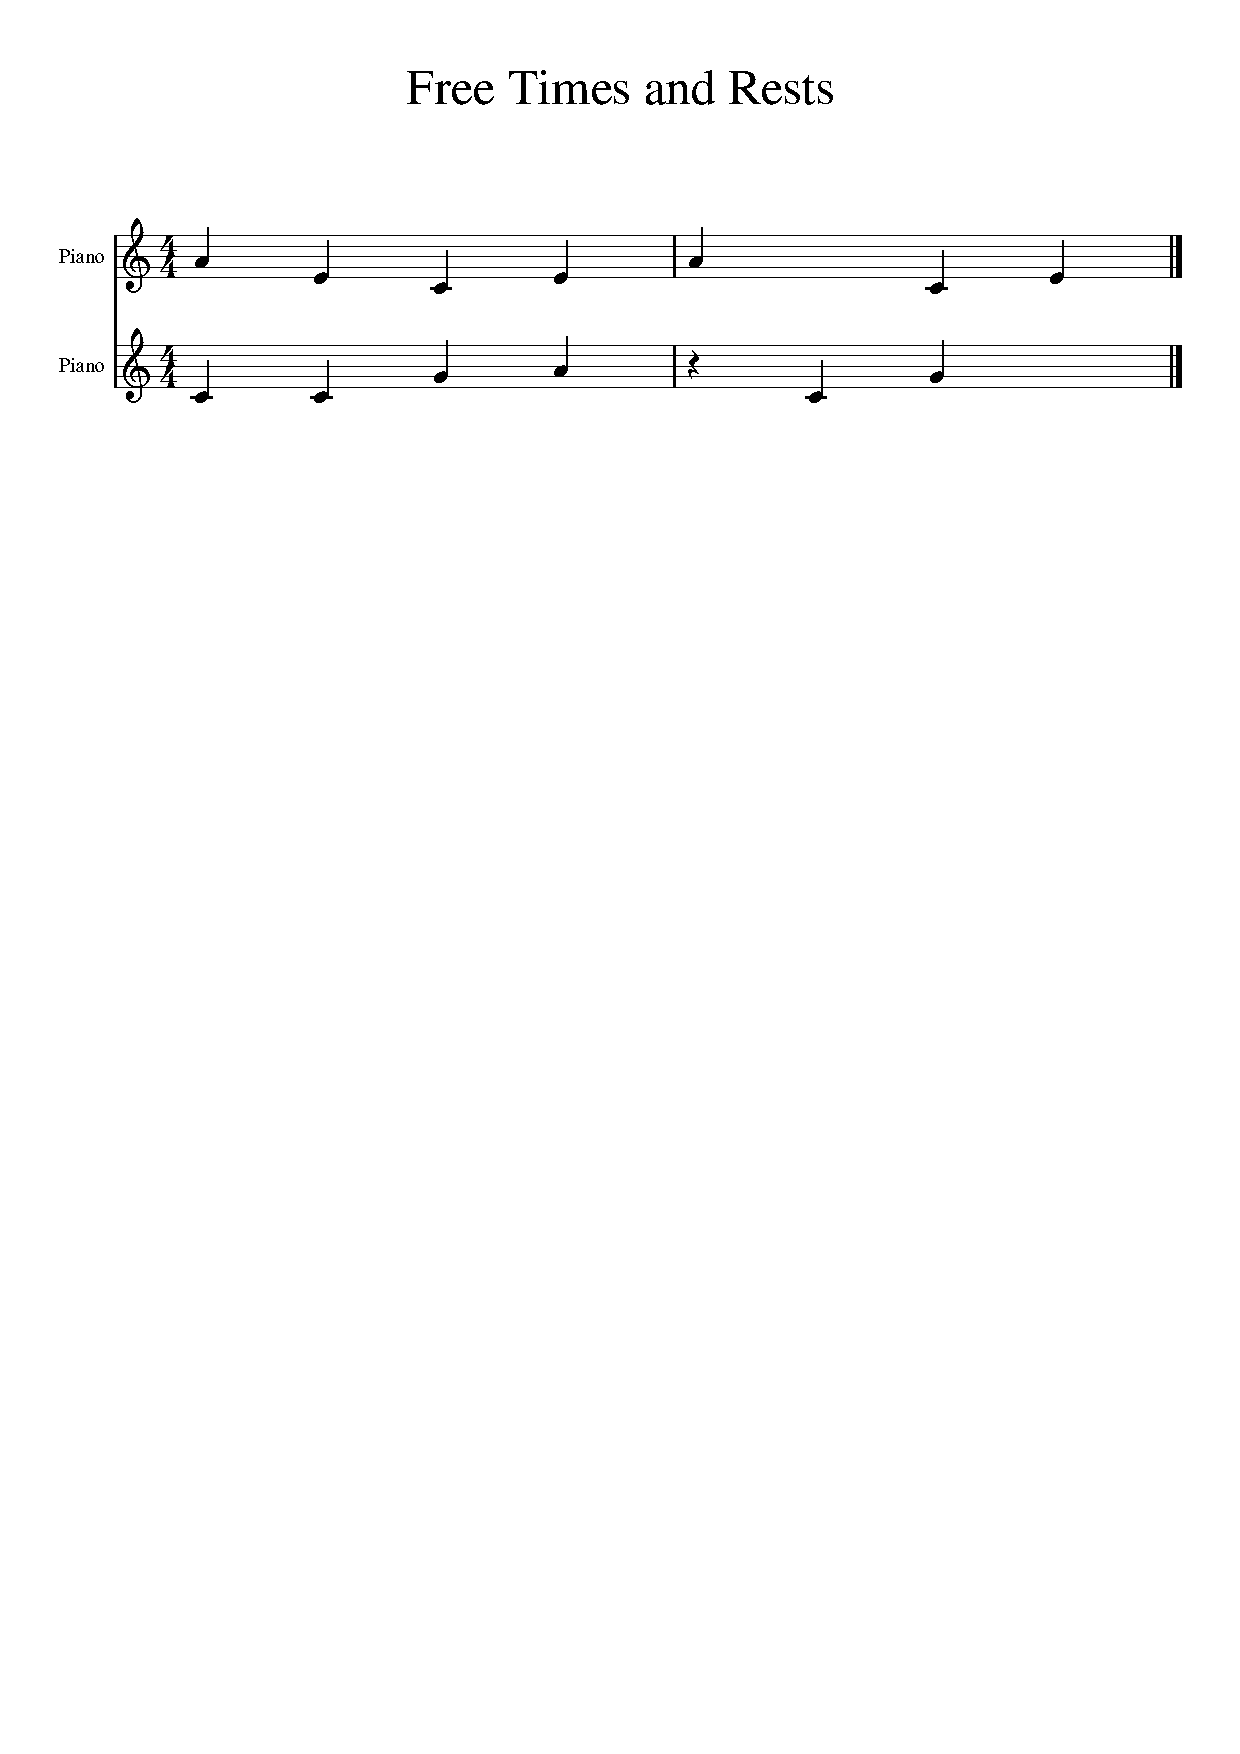
\includegraphics[width=0.8\linewidth]{imagenes/scores/freetimerests.pdf}
 	\caption{Partitura de ejemplo con algunos silencios reales y otros invisibles}
 	\label{fig:rests_score}
 \end{figure}
 
  \begin{figure}
  	\centering
  	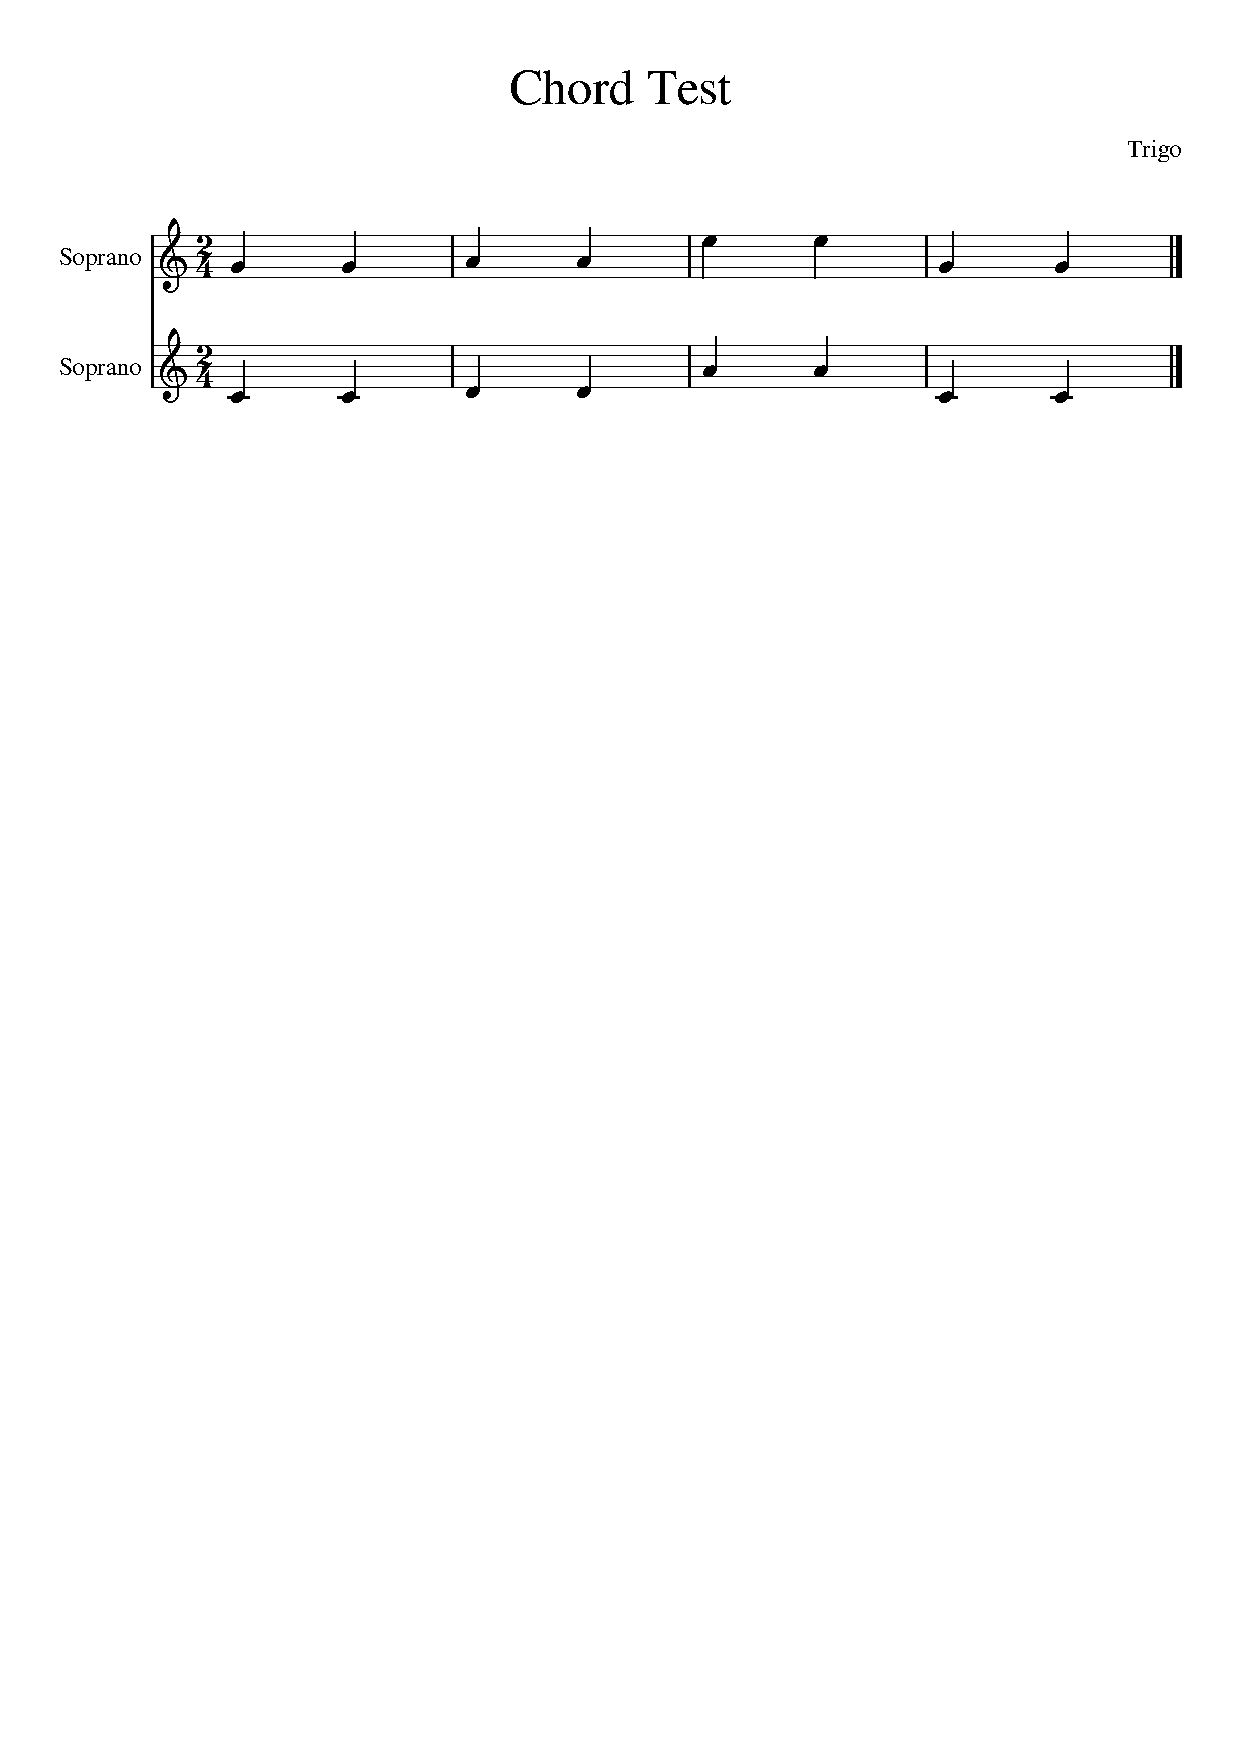
\includegraphics[width=0.8\linewidth]{imagenes/scores/Chord_Test.pdf}
  	\caption{Partitura de ejemplo con acordes definidos por la quinta para ser completada.}
  	\label{fig:chord_test}
  \end{figure}
 
\chapter{Instalación}
\label{chap:installation}
Se recomienda la instalación de la herramienta en un sistema operativo Linux. Esto se debe a que las librerías Flex y Bison se  compilan fácilmente en dicha plataforma. No obstante se proporciona el código fuente completo, por lo tanto es posible compilarlo para otros sistemas operativos.

El requisito es tener instalado Python 2.7, las ultimas versiones de Flex y Bison, además de un compilador de C (gcc sirve perfectamente). Además es necesario descargar tanto gringo 3.0.5 como clingo 3.0.5 de la página en Sourceforge del grupo Potassco\cite{potasscoweb} y el módulo Music21 en su versión 2.1.2 o superior de la página de la librería. Todas estas herramientas, compiladores y librerías deben ser accesibles mediante en el \texttt{PATH} del sistema operativo.

La instalación de tanto gringo como clingo no tiene mayor complicación, sólo deben ubicarse en alguna carpeta accesible y añadir dicha ruta al \texttt{PATH}. En la página web de Music21\cite{music21web} se incluyen instrucciones para su instalación automatizada en el sistema. Se aconseja, no obstante instalar primero diferentes herramientas para transformación y visualización o reproducción de los diferentes formatos (Léase PDF, MIDI, Lilypond, etc.) ya que de este modo, la instalación de Music21 las reconocerá y podrán ser usadas sin configuración posterior. Si se desean cambiar las preferencias sobre estas herramientas vinculadas a Music21, ha de editarse el fichero \texttt{.music21rc} presente en la carpeta \texttt{home} del usuario activo del sistema.
	
Se recomienda la instalación de un editor de partituras para poder manipular correctamente los ficheros de entrada y salida de la herramienta, esto es opcional, pero resulta conveniente. En el desarrollo se ha utilizado MuseScore 2 al ser \textit{OpenSource} y gratuito, pero cualquier editor que pueda importar y exportar ficheros en formato MusicXML servirá.

Con la herramienta, además del código fuente, se ofrece el procesador MusicXML a hechos lógicos precompilado, si no funcionase este archivo siempre puede compilarse el mencionado código fuente haciendo uso del archivo Makefile presente en la carpeta \texttt{parser/source}. un simple comando \texttt{make} desde esa ruta es suficiente. El archivo binario compilado del procesador debe estar presente en la carpeta \texttt{parser} para que la herramienta funcione correctamente.

\chapter{Manual de uso}
\label{chap:usage}
Esta herramienta está pensada para ser usada desde la línea de comandos en sistemas operativos Linux. El comando básico para su ejecución es \texttt{python haspie.py <fichero.xml>} y las opciones que permite la herramienta, junto con una pequeña explicación de cada una de ellas, pueden ser invocadas mediante la opción \texttt{-h}, como es habitual. No obstante se detalla una ejecución completa a modo de guía de uso.

\begin{Verbatim}[frame=single,fontsize=\relsize{-1}]
usage: haspie.py [-h] [-n N] [-s S] [-v V [V ...]] [-S] [-f xml|pdf|midi|ly]
                 [-o output/dir/for/file] [-t T] [-k A~G+-?] [-m major|minor]
                 [-M] [-6] [-a] [-O O] [-c config_file_name.lp]
                 XML_SCORE
haspie - Harmonizing music with ASP
positional arguments:
  XML_SCORE             input musicXML score for armonizing
optional arguments:
  -h, --help            show this help message and exit
  -n N, --num_sols N    max number of ASP solutions, by default all of them
  -s S, --span S        horizontal span to consider while harmonizing, this
                        takes in account subdivision, by default 1
  -v V [V ...], --voices V [V ...]
                        extra instruments, these can be input by name or by
                        numerical note range (i.e soprano,guitar,(65,90)...)
                        to leave one of the sides of the range unespecified
                        use 0
  -S, --show            show result in editor instead of writing it to a file
                        in the desired format
  -f xml|pdf|midi|ly, --format xml|pdf|midi|ly
                        output file format for the result
  -o output/dir/for/file, --output output/dir/for/file
                        output file name for the result
  -t T, --timeout T     maximum time (in seconds) allowed to search for
                        optimum when searching for all optimums, by default
                        there is no time limit
  -k A~G+-?, --key A~G+-?
                        key in which the score should be harmonized, if not
                        specified, parser will autodetect it
  -m major|minor, --mode major|minor
                        mode of the scale, if not specified, parser will
                        autodetect it
  -M, --melodious       turns on melodic preferences in ASP for a more melodic
                        result
  -6, --sixthslink      turns on sixth-four chord linking in ASP for a more
                        natural result (very heavy)
  -a, --all_optimums    turns on the search for all optimums when completing
                        and not just the first found, disabled by default
  -O O, --max_optimums O
                        max number of optimum solutions to display in score
                        completion, by default it's 10
  -c config_file_name.lp, --config config_file_name.lp
                        reads preference order and weights for parameters from
                        the desired *.lp file stored in /pref folder
\end{Verbatim}

Lo primero que se debe tener en cuenta es que el fichero de entrada debe proporcionarse en formato MusicXML estándar, este tipo de ficheros son uno de los más comunes en intercambio de partituras y no es difícil encontrar la partitura que deseemos armonizar en este formato. De no ser así, casi cualquier herramienta moderna de composición musical por ordenador puede exportar archivos a este formato. Ya que durante el desarrollo del proyecto se ha usado MuseScore 2, las figuras que acompañan esta sección son capturas de esta herramienta. Para opciones similares en otros editores, consúltese el manual de cada uno.

Una vez obtenido el archivo XML que se desea armonizar y/o completar, puede invocarse el comando básico ya mencionado \texttt{haspie.py <fichero.xml>} para obtener una armonización en la que se asignará un acorde a cada tiempo subdividido de la partitura. Es sumamente importante tener en cuenta la subdivisión de las notas de la partitura ya que la herramienta, para funcionar correctamente, subdivide todas las figuras a la nota más breve. Con esta llamada se calculan automáticamente todos los parámetros de armonización de la partitura: Clave y Modo. En la misma consola de comandos se imprime una serie de datos de mayor o menor utilidad para el usuario como el título de la pieza, la clave y modo detectados así como la longitud de la nota más breve de la partitura, usada como subdivisión. 

\begin{figure}[h]
	\centering
	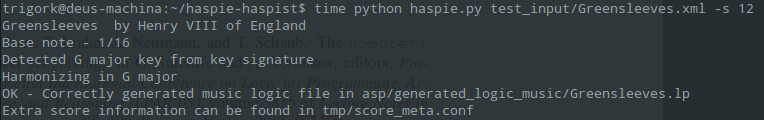
\includegraphics[width=0.8\linewidth]{imagenes/usage/metainfo.png}
	\caption{La información relevante de la partitura se muestra al comenzar la armonización}
	\label{fig:usage_metainfo}
\end{figure}

Tras la armonización se pedirá al usuario que escoja una de las soluciones propuestas por el módulo de armonización. Para esto se muestran todas numeradas y en orden inverso de optimización, siendo las últimas las mejores, de modo que el usuario solo tiene que introducir el número de aquella que desee utilizar. Si sólo se pulsa Enter, se escogerá por defecto la última ya que debería ser mejor (Aunque podría haber varias soluciones empatadas).

\begin{figure}
	\centering
	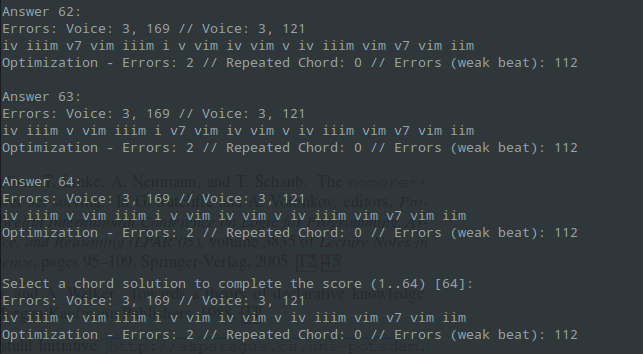
\includegraphics[width=0.8\linewidth]{imagenes/usage/harmony_select.png}
	\caption{Se pide al usuario que fije la armonización a utilizar de entre varias posibles}
	\label{fig:usage_harmony_select}
\end{figure}

A continuación se pasa al módulo de completado de partitura, ya que no se han especificado voces adicionales ni se ha modificado la partitura para contener secciones a completar, no se pedirá escoger una solución de modo similar a la armonización, al existir solo un posible resultado. Finalmente, se genera en la carpeta \texttt{out} el fichero de salida de nombre igual al de entrada, por defecto en formato MusicXML.

De todos modos las armonizaciones más frecuentes no suelen ser a tiempo si no a compás o medio compás. Para cambiar este comportamiento se puede hacer uso de la opción \texttt{-s N} donde \texttt{N} indica la cantidad de tiempos subdivididos que se tomarán en cuenta horizontalmente a la hora de asignar un acorde. Por ejemplo, en la pieza \textit{Joy to the World} se usa un compás \textbf{2/4} (es decir, dos negras por compás), pero la nota más breve de la partitura es una semicorchea, haciendo que la longitud, en semicorcheas, de este compás sea de 8. El cálculo es sencillo de realizar, solo hay que dividir la longitud fraccionaria de la nota más breve entre la longitud fraccionaria del compás y multiplicar este resultado por la cantidad de figuras originales del compás. Para este ejemplo podemos calcular $(16/4)*2=8$.

Normalmente la armadura es un buen indicativo de la clave en la que está escrita la pieza y por tanto de la tonalidad y modo en los que es correcto armonizarla, aun así estos parámetros pueden ser modificados usando \texttt{-k CLAVE} y \texttt{-m major|minor} respectivamente. 
El formato en el que se debe especificar la clave es el nombre internacional de la tonalidad (A-G) junto con un símbolo opcional \texttt{+} o \texttt{-} en caso de querer alterarla con un sostenido o un bemol respectivamente. Modificar estos parámetros alterará drásticamente la armonización de la partitura y los más probable es que si no coinciden con los detectados automáticamente producirá resultados erróneos.

Para modificar el comportamiento del módulo de completado de partituras se puede hacer uso de dos módulos de preferencias adicionales que refinan la salida para obtener un mejor resultado a cambio de requerir más tiempo de búsqueda de las soluciones. Estas preferencias tienen en cuenta las notas presentes en la entrada, pero no las modifican de ningún modo. 
El módulo de preferencias melódicas está orientado a ofrecer unas melodías más suavizadas y pulidas, principalmente minimiza la distancia de los saltos melódicos entre notas de la partitura y realiza un análisis de tendencia de las otras voces para imitar dicha tendencia. Este módulo puede ser utilizado con la opción \texttt{-M}.
El módulo de enlaces de sextas está basado en la detección y enlazado de inversiones de cuarta y sexta de acordes, muy común en polifonía. Este módulo intenta detectar estos patrones y de hallarlos busca que las nuevas notas generadas los continúen. Es significativamente costoso computacionalmente, puede ser invocado mediante la opción \texttt{-6}.

Para configurar más aún el comportamiento de ambos módulos, la importancia de cada uno de los parámetros que se maximizan o minimizan durante la búsqueda de las mejores soluciones puede ser alterada haciendo uso de ficheros de configuración en formato ASP. En la carpeta \texttt{pref} se encuentra uno comentado con las opciones por defecto. De querer hacer uso de un archivo de configuración solo hay que indicarle la ruta del mismo mediante la opción \texttt{-c /ruta/fichero/config.lp}. 

Cada parámetro de los ficheros de configuración cuenta con dos valores:
\begin{itemize}
	\item \textbf{Peso:} Indicado mediante \texttt{nombre\_weight} mide la importancia de cada uno de estos hechos en el resultado.
	\item \textbf{Prioridad:} Indicado mediante \texttt{nombrep} indica el orden en el que se ordenarán las preferencias, a más valor, mayor relevancia en el orden.
\end{itemize}

Para ajustar la cantidad de resultados puede usarse la opción \texttt{-N N}, aunque usarla limitará la búsqueda de resultados a N y no garantiza que se encuentre el mejor valor posible, de no usarse, siempre se explorará todo el espacio de búsqueda.

Para limitar la cantidad máxima de resultados óptimos mostrados por el módulo de completado de partituras puede usarse la opción \texttt{-O O}, ya que al completar puede hallarse una gran cantidad de resultados. A diferencia de \texttt{-N} esta opción solo restringe la cantidad de óptimos mostrados, independientemente de haberse limitado el espacio de búsqueda.

Para controlar el tiempo de ejecución del módulo de completado, ya que este puede dispararse al querer completar grandes secciones puede usarse la opción \texttt{-t tiempo} para expresar cuantos segundos se quiere invertir en la búsqueda. La herramienta siempre usará la cantidad de tiempo especificada, por defecto es 5 segundos.

Existen dos modos de solicitar al módulo de completado de partituras que haga su trabajo:
\begin{itemize}
	\item \textbf{Silencios Completables:} Se realiza mediante un marcado especial en el editor de partituras.
	\item \textbf{Inclusión de voces nuevas:} Se realiza desde la línea de comandos.
\end{itemize}

Los silencios completables son silencios especiales que el procesador interpreta como huecos en vez de como silencios. Para lograr esto se hace uso de una meta-propiedad de las figuras en MusicXML: Su visibilidad. Cualquier figura puede marcarse como invisible desde el panel de propiedades de la figura en el editor, con el fin de que esta no sea impresa en el momento de hacerlo. Esta herramienta entiende los silencios marcados como ``no visibles'' como huecos a rellenar y la figura utilizada para rellenar dicho espacio será la correspondiente al silencio ``no visible'' que aparecía originalmente en la partitura.

\begin{figure}[h]
	\centering
	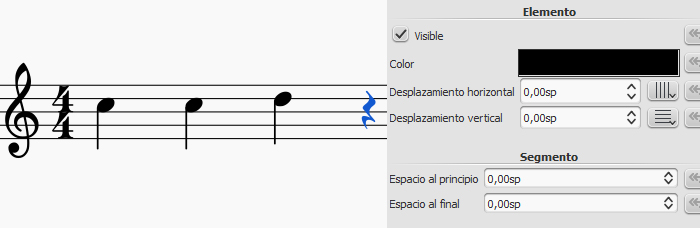
\includegraphics[width=0.8\linewidth]{imagenes/usage/select_silence.jpg}
	\caption{Seleccionando una figura podemos ver sus propiedades, entre otras la casilla de visibilidad}
	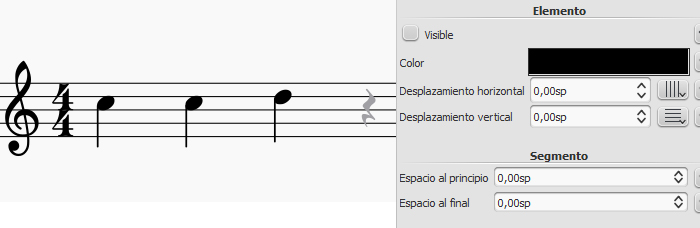
\includegraphics[width=0.8\linewidth]{imagenes/usage/invisible_silence.jpg}
	\caption{Desmarcando la casilla de visibilidad, la figura pasa a un color más claro, indicando que no es visible}
	\label{fig:invisible_silence}
\end{figure}

Las voces nuevas son líneas melódicas completamente vacías originalmente que el módulo de completado se encarga de rellenar respetando la armonía y la tesitura de la voz. Para hacer esto solo hay que usar la opción \texttt{-v voz1 [voz2]...} que toma tantas voces como se quiera añadir como parámetro. Pueden ser especificadas mediante rango de numérico de notas en la forma \texttt{min,max}, usándose 0 si quiere dejarse uno de los extremos abiertos o mediante nombre si la tesitura (o rango de notas) está definida en el fichero \texttt{asp/include/voice\_types.lp}. En éste figuran las tesituras corales más comunes, pero cualquier nuevo instrumento puede ser definido a gusto del usuario.

En caso de requerir completar la partitura de algún modo, tras la armonización, la herramienta solicitará al usuario que escoja la solución que más le guste, mostrando los errores, acordes y notas de cada una de las mejores soluciones halladas.

\begin{figure}
	\centering
	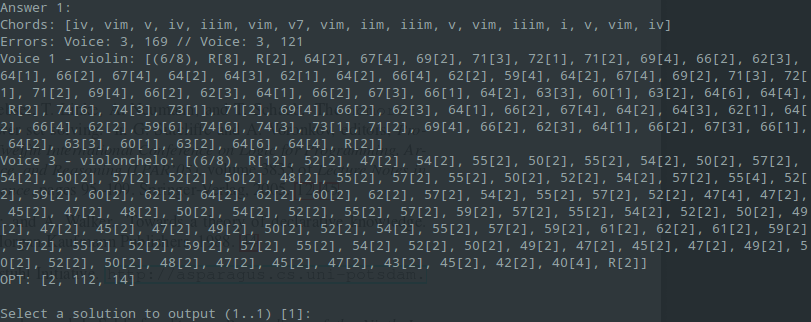
\includegraphics[width=0.8\linewidth]{imagenes/usage/completion_select.png}
	\caption{Se pide al usuario que seleccione la solución que más le guste entre varias posibles}
	\label{fig:usage_completion_select}
\end{figure}

Si se quiere obtener el fichero en algún formato de salida diferente a MusicXML este puede ser especificado mediante \texttt{-f formato}, siempre y cuando se dispongan de herramientas para realizar la conversión instaladas en el sistema. Por ejemplo, para exportar a Lilypond usando \texttt{-f ly} precisaríamos de tener instalado el propio entorno de Lilypond en el sistema. Así mismo se puede cambiar el nombre del fichero de salida con la habitual opción \texttt{-o /ruta/de/salida} (La ruta debe existir).

Por último, si no existiese interés en almacenar el fichero de salida y solo se desease previsualizar el resultado, puede usarse la opción \texttt{-S} para ello. Esto generará un fichero temporal y se ejecutará el software relacionado con la extensión seleccionada para previsualizarlo.

\newpage
\thispagestyle{empty}
